\chapter{LAB Session 03 --Capacitive feedback amplifier
based on a two-stage OTA}
\section{Initial design analysis}

\subsection{Initial transistors and DC Operating Point Verification}
% subsection was incorrect.
\begin{table}[h]
\centering
\begin{tabular}{|c|c|c|c|c|c|}
\hline
\textbf{Transistor} &
\textbf{$|V_{OV}|$ [V]} &
\textbf{L [$\mu$m]} &
\textbf{W [$\mu$m]} &
\textbf{\# Fingers} &
\textbf{$I_D$ [$\mu$A]}
\\ \hline

M1, M2 &
0.14 &
0.24 &
4 &
4 &
100.2
\\ \hline

M3, M4 &
0.21 &
0.24 &
12 &
8 &
100.2
\\ \hline

M5, M6 &
0.22 &
0.24 &
48 &
24 &
444.2
\\ \hline

M7, M8 &
0.13 &
0.24 &
19.2 &
16 &
444.2
\\ \hline

M9A, M9B &
0.13 &
0.24 &
4.8 &
4 &
100.2
\\ \hline

M10, M11 &
0.21 &
0.24 &
6 &
4 &
53.56
\\ \hline

M12 &
0.13 &
0.24 &
2.4 &
2 &
53.56
\\ \hline

\end{tabular}
\caption{Initial transistor sizing of the fully differential two-stage OTA.}
\label{tab:ota_initial_sizing}
\end{table}


\begin{figure}[H]
    \centering
    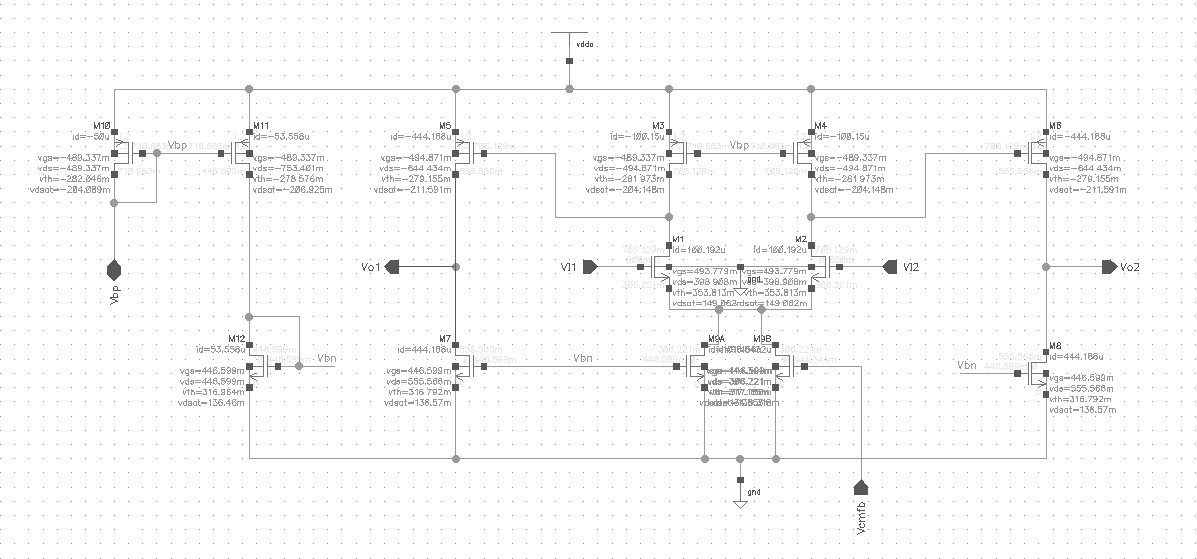
\includegraphics[width=1.0\textwidth]{Images_part3/TS_OTA_OL_OP.png}
    \caption{DC operating point of the initial OTA design.}
    \label{fig:initial_ota_operating_point}
\end{figure}
The operating point simulation confirms that all transistors are correctly biased in saturation region. Moreover, the common-mode output voltage settles close to the desired value, indicating a correct operation of the common-mode feedback network.
\subsection{Open-Loop OTA Analysis}
\begin{figure}[H]
    \centering
    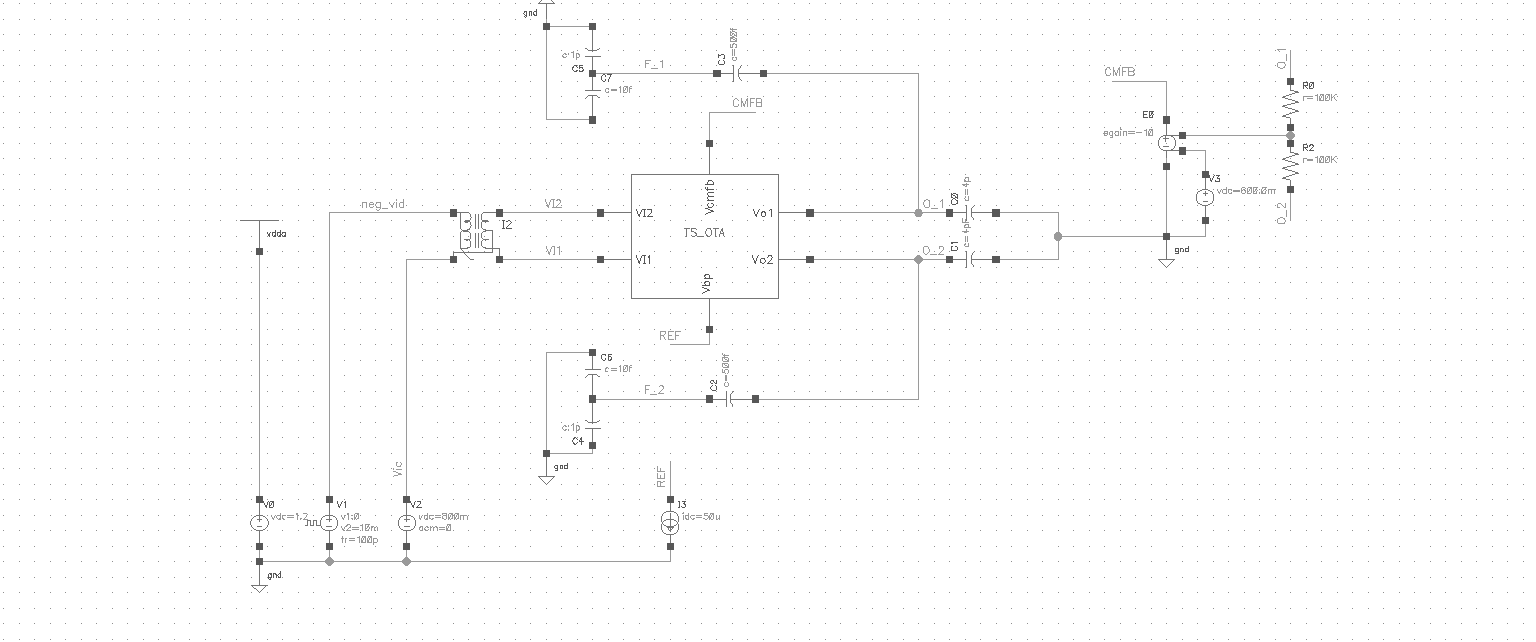
\includegraphics[width=1.0\textwidth]{Images_part3/OL_TESTBENCH.png}
    \caption{Open-loop testbench used for loop transfer function characterization.}
    \label{fig:tb_ol}
\end{figure}
The open-loop characterization of the OTA was performed using the testbench shown in Fig.~\ref{fig:tb_ol}. The capacitive feedback network was disconnected from the OTA input in order to evaluate the loop transfer function and assess the intrinsic stability of the amplifier.
The feedback factor
\[
\beta=\frac{C_F}{C_F+C_S+C_I}\approx0.33
\]
represents the fraction of the output signal fed back to the OTA input through the capacitive network. It therefore determines the loop transfer function
\[
T(s)=\beta A_{OL}(s),
\]
and directly affects the stability and phase margin of the closed-loop system. $A_{OL}(s)$ is the open-loop differential gain of the OTA. Using this setup, the Bode plots and transient responses reported in the following section were extracted.


\begin{figure}[H]
    \centering
    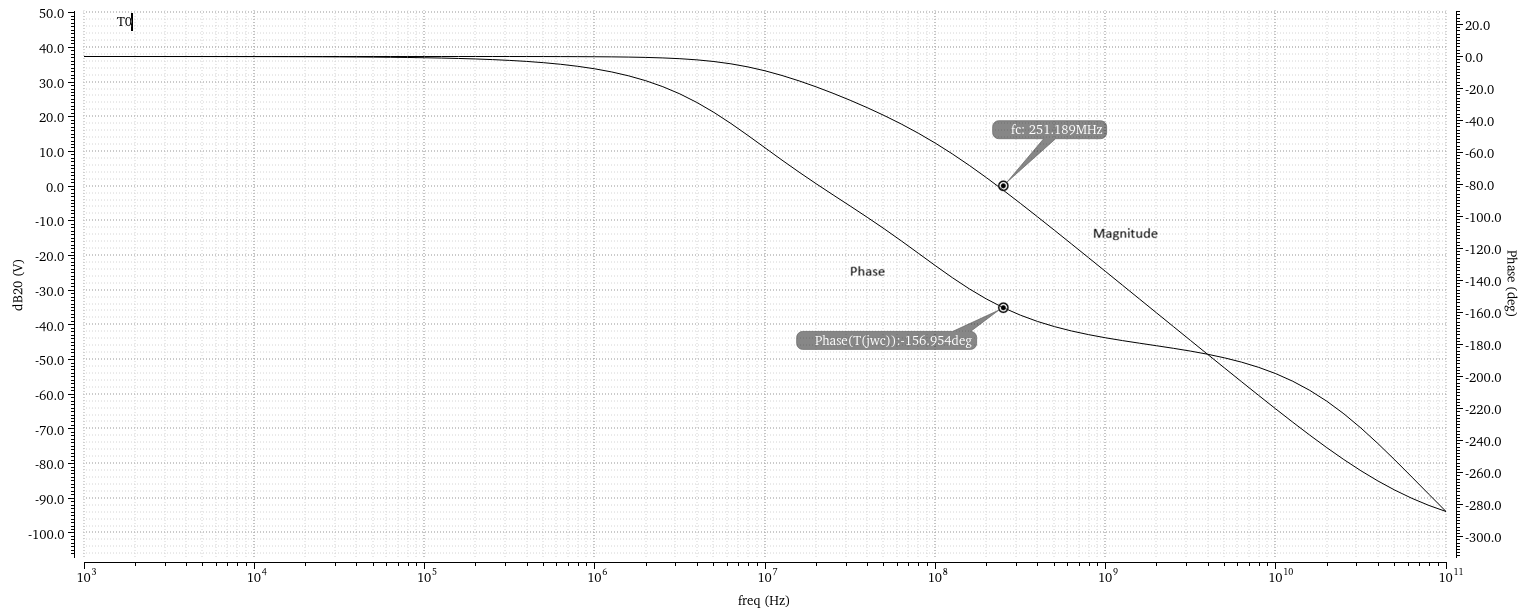
\includegraphics[width=1.0\textwidth]{Images_part3/T0_bodeplt.png}
    \caption{Bode plot of the open-loop transfer function.}
    \label{fig:open_loop_bode}
\end{figure}
The initial loop transfer function exhibits a low-frequency gain of $T_0\approx37.8\,\mathrm{dB}$, a crossover frequency of $f_c\approx251\,\mathrm{MHz}$, and a phase margin of only $PM\approx23^\circ$. Although the bandwidth is relatively high, the poor phase margin indicates insufficient stability and makes the circuit unsuitable for closed-loop operation. Therefore, frequency compensation is required.
\subsection{Transient response of the differential and common mode signal}


\begin{figure}[H]
    \centering
    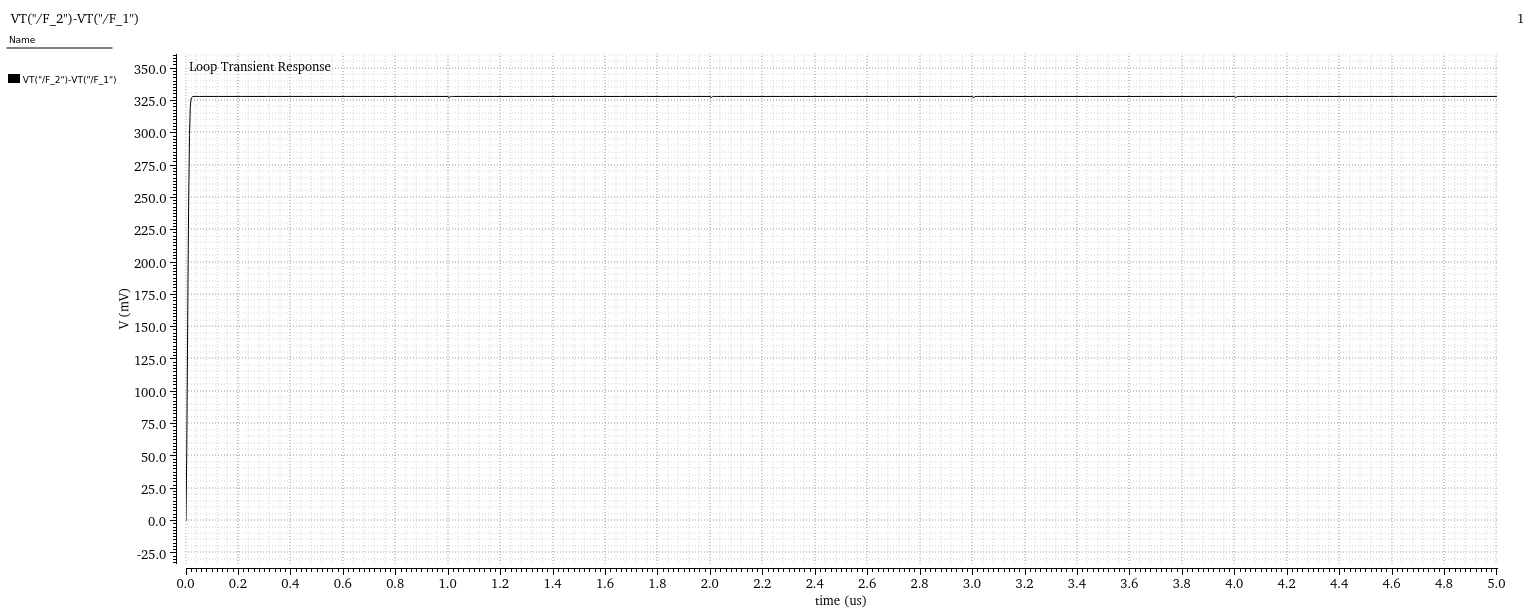
\includegraphics[width=1.0\textwidth]{Images_part3/loop_tran_resp.png}
    \caption{Transient response of the loop differential output signal.}
    \label{fig:open_loop_transient}
\end{figure}
The differential transient response confirms the high gain and bandwidth of the uncompensated OTA. A small differential input step produces a large output variation, consistent with the large open-loop gain previously observed in the frequency-domain analysis.


\begin{figure}[H]
    \centering
    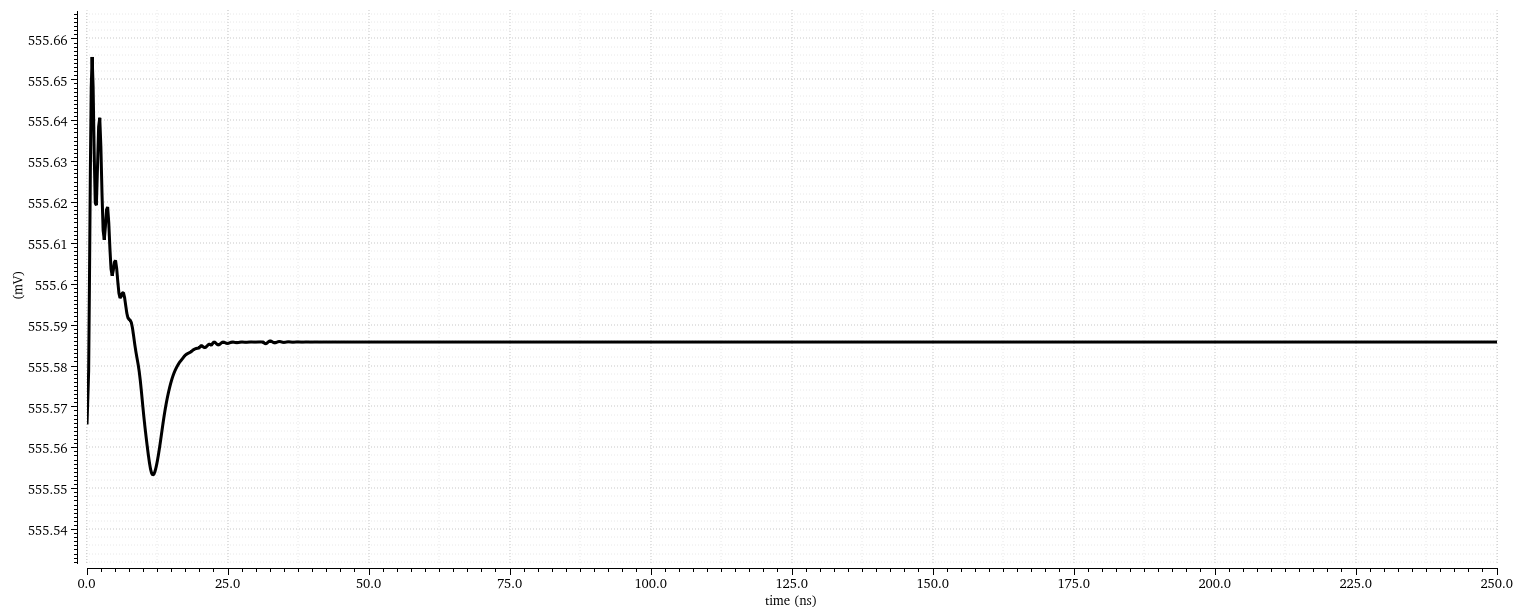
\includegraphics[width=1.0\textwidth]{Images_part3/OL_tran_cm.png}
    \caption{Transient response of the loop common-mode output component.}
    \label{fig:open_loop_common_mode_transient}
\end{figure}
The common-mode transient response confirms effective CMFB loop operation. After a minimal overshoot of $\Delta V_{OCM}\approx 0.1\,\mathrm{mV}$, the output common-mode voltage rapidly settles to $V_{OCM}\approx 556\,\mathrm{mV}$, demonstrating stable regulation and precise control of the common-mode level.

\subsection{Closed-Loop Feedback Amplifier Analysis}

\begin{figure}[H]
    \centering
    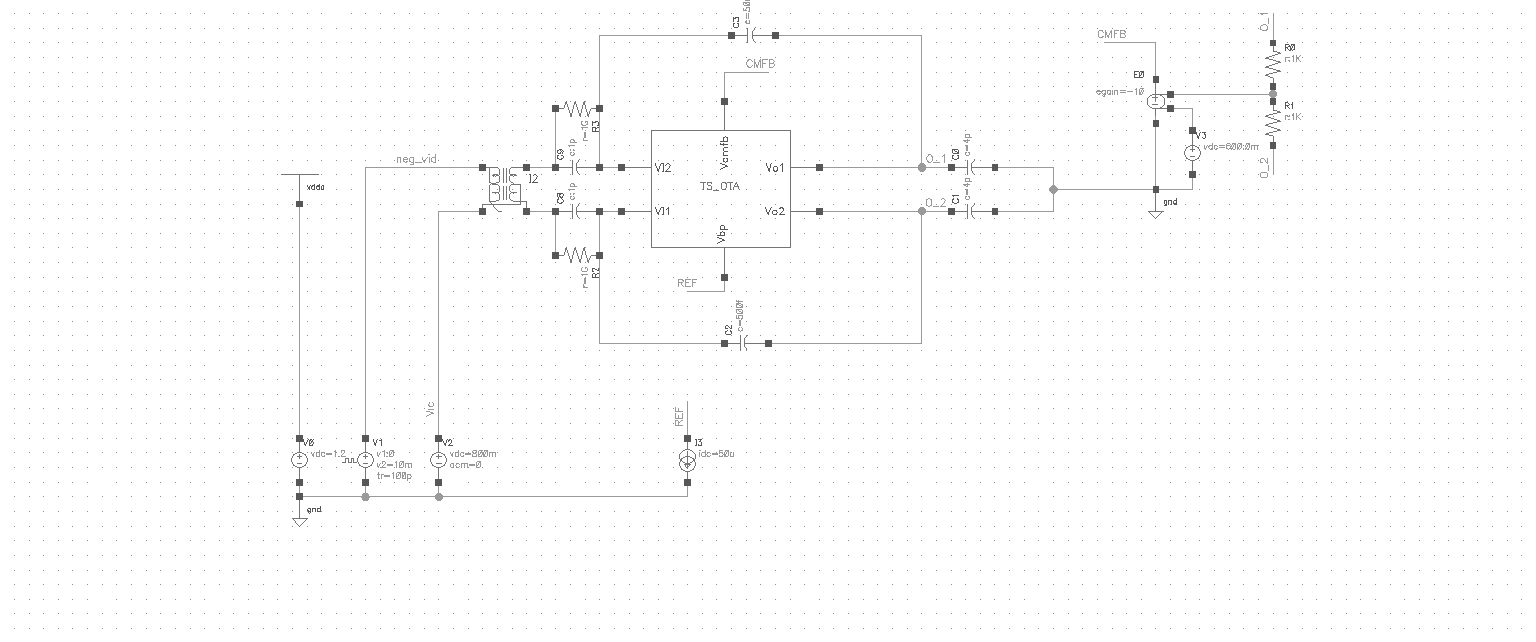
\includegraphics[width=1.0\textwidth]{Images_part3/cl3_TESTBENCH.png}
    \caption{Closed-loop testbench used for capacitive feedback amplifier characterization.}
    \label{fig:tb_cl}
\end{figure}
The closed-loop behavior of the capacitive feedback amplifier was analyzed using the testbench shown in Fig.~\ref{fig:tb_cl}. In this configuration, the capacitive feedback network is connected around the OTA, thus establishing the differential closed-loop gain through the capacitor ratio.

Assuming an ideal OTA with sufficiently large loop gain, the low-frequency closed-loop gain is

\[
A_{CL,\mathrm{ideal}}
=
-\frac{C_S}{C_F}
=
-2.
\]
The large input resistors are used to impose the input common-mode voltage without significantly affecting the ac response of the capacitive network. The testbench also includes the external load capacitances and the ideal common-mode feedback circuit in order to reproduce the intended operating conditions of the amplifier.

Using this setup, the closed-loop frequency response and transient step response of the feedback amplifier were extracted and analyzed.
\begin{figure}[H]
    \centering
    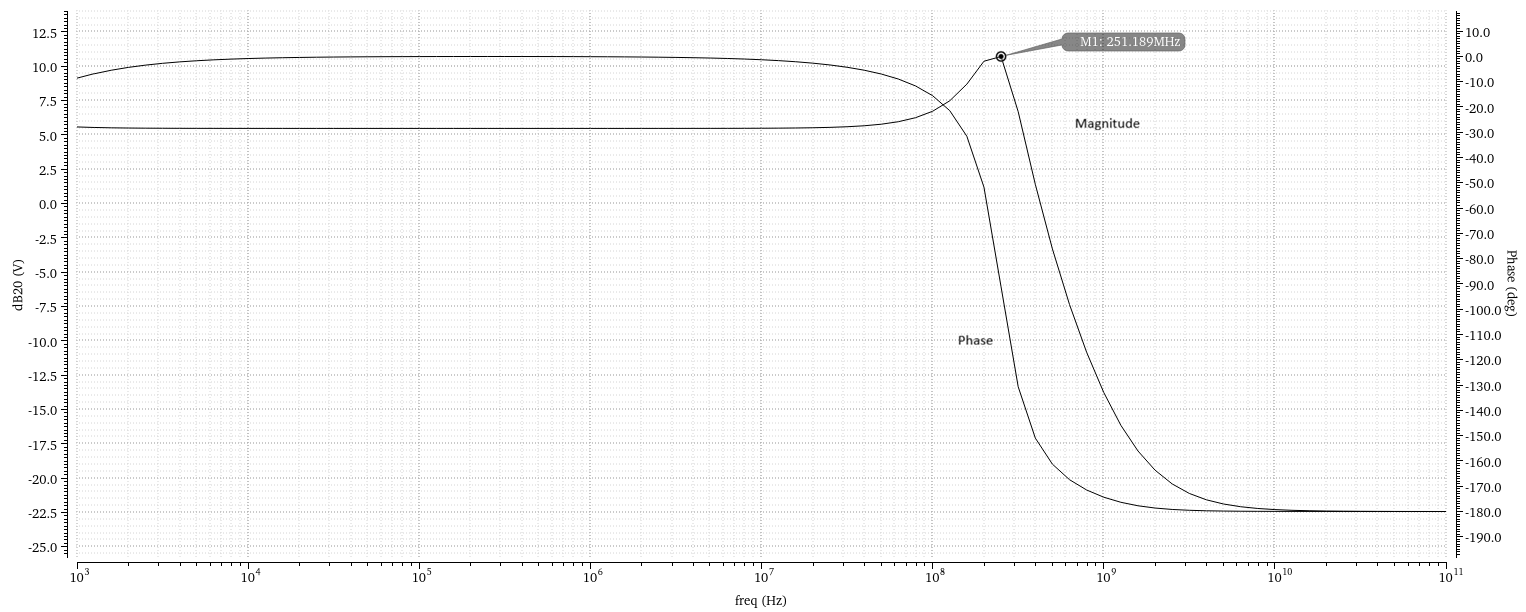
\includegraphics[width=1.0\textwidth]{Images_part3/CL_bodeplt.png}
    \caption{Bode plot of the closed-loop differential transfer function.}
    \label{fig:closed_loop_bode}
\end{figure}
The closed-loop differential transfer function exhibits a low-frequency gain of approximately

\[
A_{CL,0}\approx5.2\,\mathrm{dB},
\]

which is close to the ideal value expected from the capacitive feedback network.

However, a pronounced resonant peak is clearly visible around the bandwidth frequency, indicating a strongly underdamped closed-loop response. This behavior is consistent with the low phase margin previously extracted from the loop transfer function.


\subsection{Transient response of the differential mode signal}
\begin{figure}[H]
    \centering
    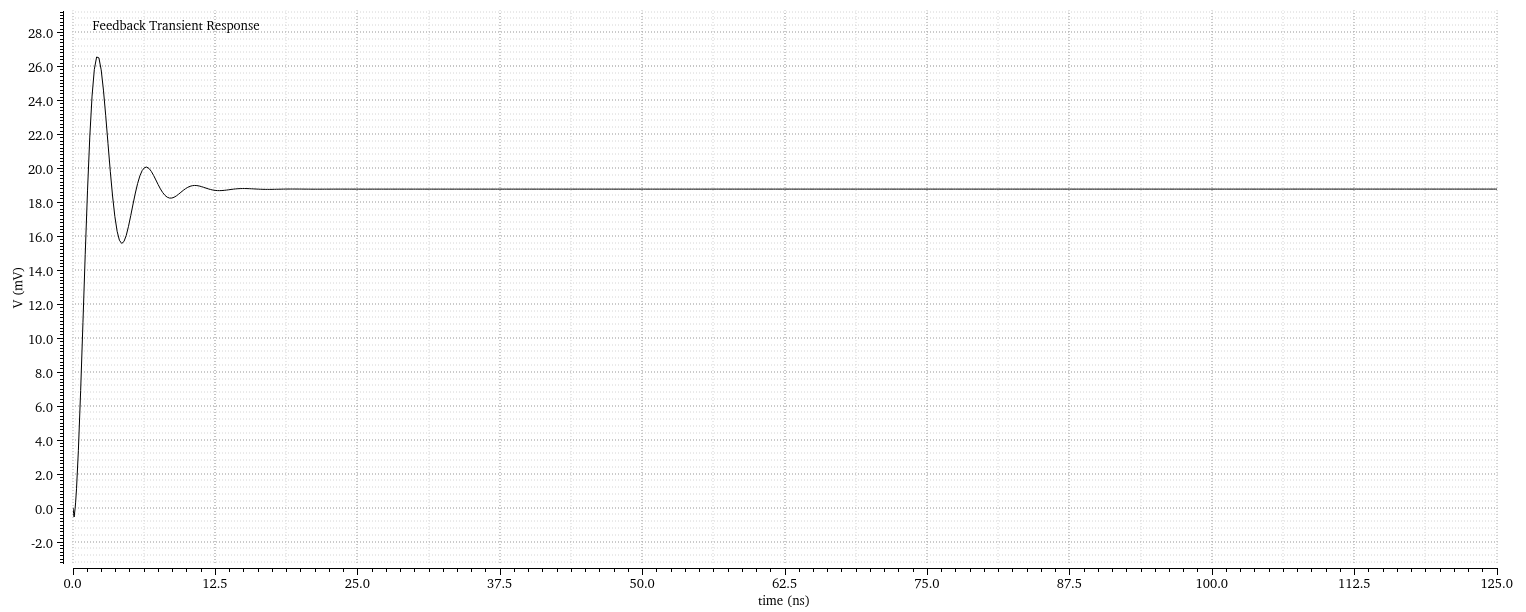
\includegraphics[width=1.0\textwidth]{Images_part3/Feed_tran_resp_doppia.png}
    \caption{Transient step response of the closed-loop differential output signal.}
    \label{fig:closed_loop_transient}
\end{figure}
The closed-loop differential step response confirms the poor stability predicted by the initial loop-transfer analysis ($PM \approx 23^\circ$). Consequently, the output exhibits severe ringing and a large overshoot, reaching a peak value of $v_{o,\mathrm{peak}} \approx 26.3\,\mathrm{mV}$ before settling toward a steady-state value of $v_o(\infty) \approx 18.9\,\mathrm{mV}$.



\section{OTA Redesign}
\subsection{First-Order Hand Design of the OTA}
The redesign process starts from the dynamic error specification. Assuming a first-order closed-loop response, the dynamic error is approximated as:
\begin{equation*}
\varepsilon_d(t_s)\simeq e^{-\omega_c t_s}
\end{equation*}
Imposing a settling error below $0.2\%$ after $20\,\mathrm{ns}$ yields:
\begin{align*}
\varepsilon_d(t_s) \leq 0.002 \implies \omega_c \geq \frac{-\ln(0.002)}{20\,\mathrm{ns}} \simeq 310\,\mathrm{Mrad/s} \implies f_c = \frac{\omega_c}{2\pi} \simeq 49.5\,\mathrm{MHz}
\end{align*}
Consequently, the OTA target crossover frequency is set to \boxed{f_c\simeq50\,\mathrm{MHz}}.

To satisfy the power constraint, the differential pair and second-stage transistors are biased at $I_{D1}=I_{D5}=225\,\mu\mathrm{A}$, with a total current consumption of:
\begin{equation*}
I_{TOT} = 2I_{REF}+2I_{D1}+2I_{D5} = 2\cdot50 + 2\cdot225 + 2\cdot225 = 1\,\mathrm{mA}
\end{equation*}
Overdrive voltages are chosen as $V_{OV1}=V_{OV5}=0.15\,\mathrm{V}$ and $V_{OV3}=V_{OV7}=V_{OV9}=V_{OV10}=V_{OV11}=V_{OV12}=0.3\,\mathrm{V}$. The resulting transconductance for the driving transistors is:
\begin{equation*}
g_{m1}=g_{m5} = \frac{2I_D}{V_{OV}} = \frac{2\cdot225\,\mu\mathrm{A}}{0.15\,\mathrm{V}} = 3\,\mathrm{mS}
\end{equation*}

The static error spec requires $\varepsilon_0 \simeq \frac{1}{1+T_0} \leq 0.002$, where $T_0=\beta A_{dd0}$ and $\beta=0.33$, hence $A_{dd0} \geq \frac{499}{0.33} \simeq 1512$. To ensure design margin, a larger open-loop gain target is adopted:
\begin{equation*}
A_{dd0} \simeq g_{m1}g_{m5}R_1R_2 \simeq 2025
\end{equation*}
Assuming $R_1=R_2=15\,\mathrm{k}\Omega$ (where $R_1=r_{o1}\parallel r_{o3}$ and $R_2=r_{o5}\parallel r_{o7}$), the estimated gain is verified:
\begin{equation*}
A_{dd0} = (3\,\mathrm{mS})^2 \cdot (15\,\mathrm{k}\Omega)^2 \simeq 2025
\end{equation*}
Assuming symmetric output resistances $r_{o1}=r_{o3}=r_{o5}=r_{o7}=30\,\mathrm{k}\Omega$, the channel lengths are estimated via $r_o=\frac{\eta L}{I_D} \implies L=\frac{r_o I_D}{\eta}$:
\begin{align*}
L_n &= \frac{30\,\mathrm{k}\Omega\cdot225\,\mu\mathrm{A}}{1.1\cdot10^7} \simeq 0.61\,\mu\mathrm{m} \implies L_1=L_7=L_9=L_{12}\simeq0.61\,\mu\mathrm{m} \\
L_p &= \frac{30\,\mathrm{k}\Omega\cdot225\,\mu\mathrm{A}}{1.5\cdot10^7} \simeq 0.45\,\mu\mathrm{m} \implies L_3=L_5=L_{10}=L_{11}\simeq0.45\,\mu\mathrm{m}
\end{align*}
Transistor widths are calculated using $W = \frac{2I_D L}{k'V_{OV}^2}$, matching the current-mirror ratios $\frac{W_3}{W_{10}} = \frac{W_7}{W_{12}} = \frac{225}{50} = 4.5$. The final hand-estimated dimensions are summarized in Table~\ref{tab:redesign_hand_sizing}.

\begin{table}[H]
\centering
\caption{Hand-estimated transistor dimensions for the redesigned OTA.}
\label{tab:redesign_hand_sizing}
\begin{tabular}{|c|c|c|c|c|}
\hline
\textbf{Transistor} & \textbf{$V_{OV}$ [V]} & \textbf{L [$\mu$m]} & \textbf{W [$\mu$m]} & \textbf{$I_D$ [$\mu$A]} \\ \hline
M1, M2 & 0.15 & 0.61 & 26.1 & 225 \\ \hline
M3, M4 & 0.30 & 0.45 & 22.5 & 225 \\ \hline
M5, M6 & 0.15 & 0.45 & 90.0 & 225 \\ \hline
M7, M8 & 0.30 & 0.61 & 6.53 & 225 \\ \hline
M9A, M9B & 0.30 & 0.61 & 6.53 & 225 \\ \hline
M10, M11 & 0.30 & 0.45 & 5.0 & 50 \\ \hline
M12 & 0.30 & 0.61 & 1.45 & 50 \\ \hline
\end{tabular}
\end{table}

Under dominant-pole conditions, the closed-loop bandwidth is $f_{BW,CL}\approx\beta\cdot GBW$, requiring a minimum $GBW \simeq \frac{50\,\mathrm{MHz}}{0.33} \simeq 150\,\mathrm{MHz}$. To account for non-idealities observed in previous iterations, a conservative target of $GBW\simeq300\,\mathrm{MHz}$ is chosen. The compensation capacitor is:
\begin{equation*}
GBW=\frac{g_{m1}}{2\pi C_C} \implies C_C = \frac{3\,\mathrm{mS}}{2\pi\cdot300\,\mathrm{MHz}} \simeq 1.6\,\mathrm{pF}
\end{equation*}
To improve the phase margin ($PM$), a nulling resistor $R_Z$ compensates the non-dominant pole:
\begin{equation*}
PM = 90.1^\circ - \tan^{-1}\left(\beta\frac{g_{m1}}{g_{m5}}\frac{C_L}{C_C}\right) + \tan^{-1}\left(\beta\frac{g_{m1}}{g_{m5}}k\right)
\end{equation*}
From this, the zero-position parameter is $k\simeq1.376$, yielding:
\begin{equation*}
R_Z = \frac{1+k}{g_{m5}} = \frac{1+1.376}{3\,\mathrm{mS}} \simeq 790\,\Omega \approx 800\,\Omega
\end{equation*}
These values served as the initial design point for subsequent Cadence simulations.

\subsection{Simulation-Based Optimization of the Initial OTA Design}

Although the analytical design satisfied first-order specifications, non-ideal effects neglected in the simplified hand calculations introduced discrepancies between theoretical predictions and simulated performance.

In the initial simulation iterations, the low-frequency gain was significantly lower than targeted. To counteract this, the channel lengths of the transistors dictating the gain of both stages (\(M_1\), \(M_3\), \(M_5\)) and the corresponding bias-current mirrors were progressively increased. This adjustment enhanced the equivalent output resistances:
\[
R_1=r_{o1}\parallel r_{o3}, \qquad R_2=r_{o5}\parallel r_{o7}
\]
Simultaneously, the transistor widths were rescaled to preserve the design overdrive voltages and bias currents.

Once the loop-gain target was secured, the optimization focused on the compensation network. The compensation capacitor \(C_C\) and the nulling resistor \(R_Z\) were iteratively tuned to suppress the phase degradation from non-dominant poles and maximize the phase margin. The final optimized compensation values are:
\[
\boxed{C_C=2.61\,\mathrm{pF}}, \qquad \boxed{R_Z=1.7\,\mathrm{k}\Omega}
\]

The final transistor dimensions and layout configurations resulting from the simulation-based refinement are summarized in Table~\ref{tab:final_ota_sizing4}.

\begin{table}[H]
\centering
\begin{tabular}{|c|c|c|}
\hline
\textbf{Transistor} & \textbf{L [$\mu$m]} & \textbf{W [$\mu$m]} \\ \hline
M1, M2    & 0.96 & 40.8  \\ \hline
M3, M4    & 1.2  & 60    \\ \hline
M5, M6    & 1.2  & 240   \\ \hline
M7, M8    & 0.96 & 10.2  \\ \hline
M9A, M9B & 0.96 & 10.2  \\ \hline
M10, M11 & 1.2  & 13.34 \\ \hline
M12       & 0.96 & 2.27  \\ \hline
\end{tabular}
\caption{Final optimized OTA transistor sizing after simulations.}
\label{tab:final_ota_sizing4}
\end{table}

\subsection{DC Operating Point Verification}
The final OTA DC operating point is reported in Fig.~\ref{fig:dc_op_point}. All transistors operate in saturation, validating the small-signal biasing conditions.

\begin{figure}[H]
    \centering
    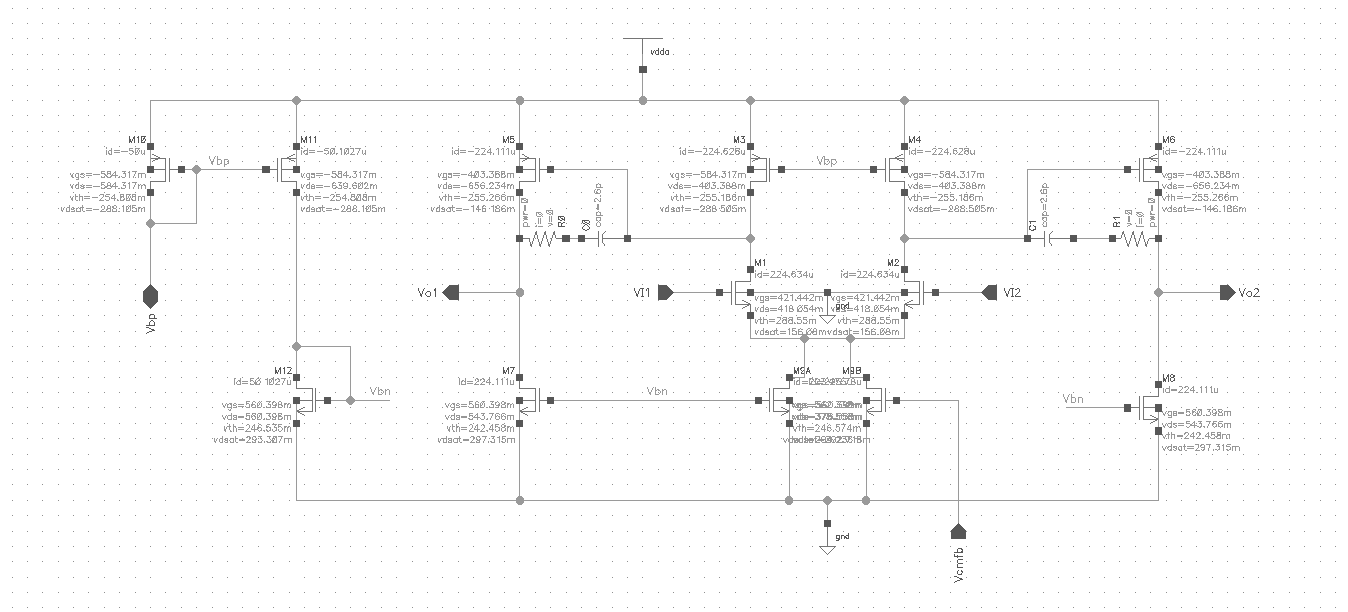
\includegraphics[width=0.9\textwidth]{immaginicorrettereport3/DC_OP_POINT.png}
    \caption{DC operating point of the final OTA design.}
    \label{fig:dc_op_point}
\end{figure}

The simulated branch currents are $I_D \simeq 224.6\,\mu\mathrm{A}$, $I_{D5}\simeq224.1\,\mu\mathrm{A}$, and $I_{REF}=50\,\mu\mathrm{A}$, yielding a total current consumption of:
\[
I_{TOT}=2I_{REF}+2I_D+2I_{D5} \simeq 997\,\mu\mathrm{A}
\]
This satisfies the power constraint $I_{TOT}<1\,\mathrm{mA}$. With $V_{DD}=1.2\,\mathrm{V}$, the resulting DC power consumption is:
\[
P_{DC}=V_{DD}I_{TOT} \simeq 1.20\,\mathrm{mW}
\]

\subsection{Loop Transfer Function Analysis}

The Bode plot of the loop transfer function (Fig.~\ref{fig:loop_gain}) is used to extract the low-frequency loop gain, crossover frequency, and phase margin.

\begin{figure}[H]
    \centering
    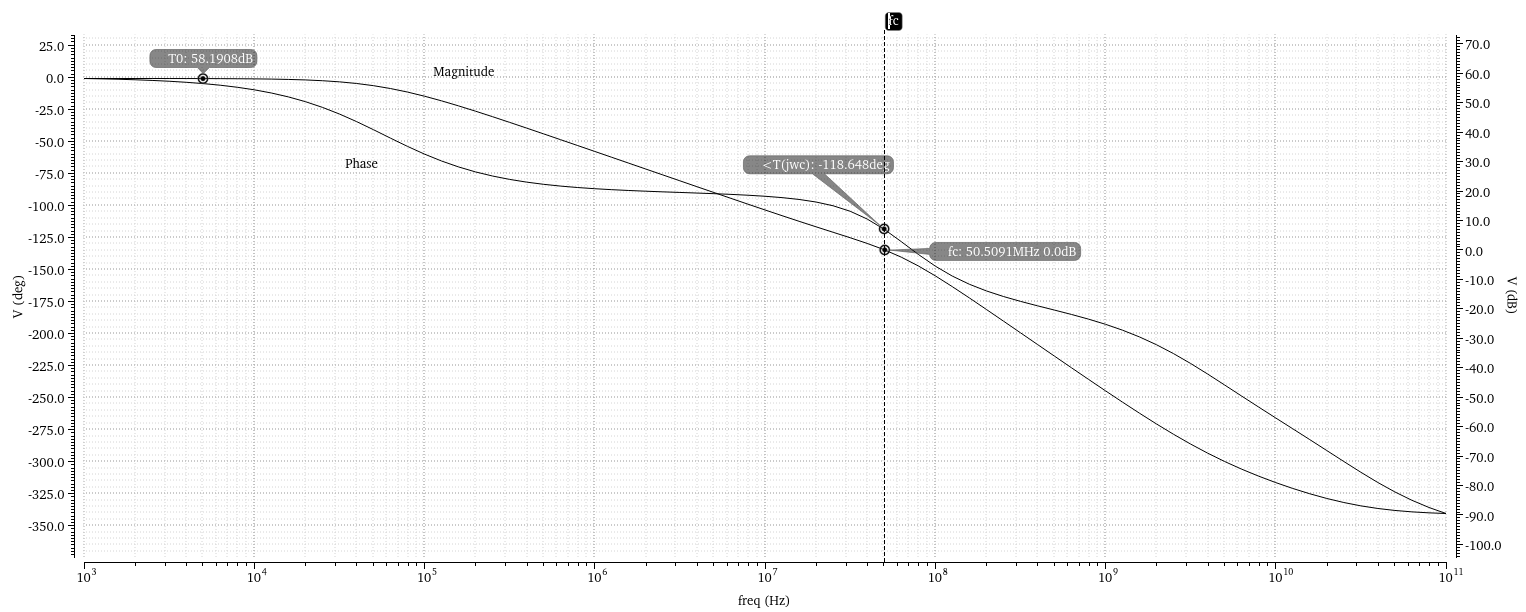
\includegraphics[width=0.85\textwidth]{immaginicorrettereport3/LOOPGAIN.png}
    \caption{Bode plot of the final loop transfer function.}
    \label{fig:loop_gain}
\end{figure}

The simulation yields $T_0=58.19\,\mathrm{dB}$, $f_c=50.51\,\mathrm{MHz}$, and $\angle T(j\omega_c)=-118.65^\circ$. The phase margin is thus calculated as:
\[
PM=180^\circ+\angle T(j\omega_c) = 180^\circ-118.65^\circ \simeq 61.35^\circ
\]
which satisfies the design specification ($60^\circ \leq PM \leq 70^\circ$).

Fig.~\ref{fig:loop_transient} shows the open-loop differential return signal $V_T(F_2)-V_T(F_1)$. The signal settles around $353\,\mathrm{mV}$, consistent with the low-frequency loop gain after the capacitive feedback network. Since the loop is opened for testbench analysis, this transient does not reflect the closed-loop settling behavior.

\begin{figure}[H]
    \centering
    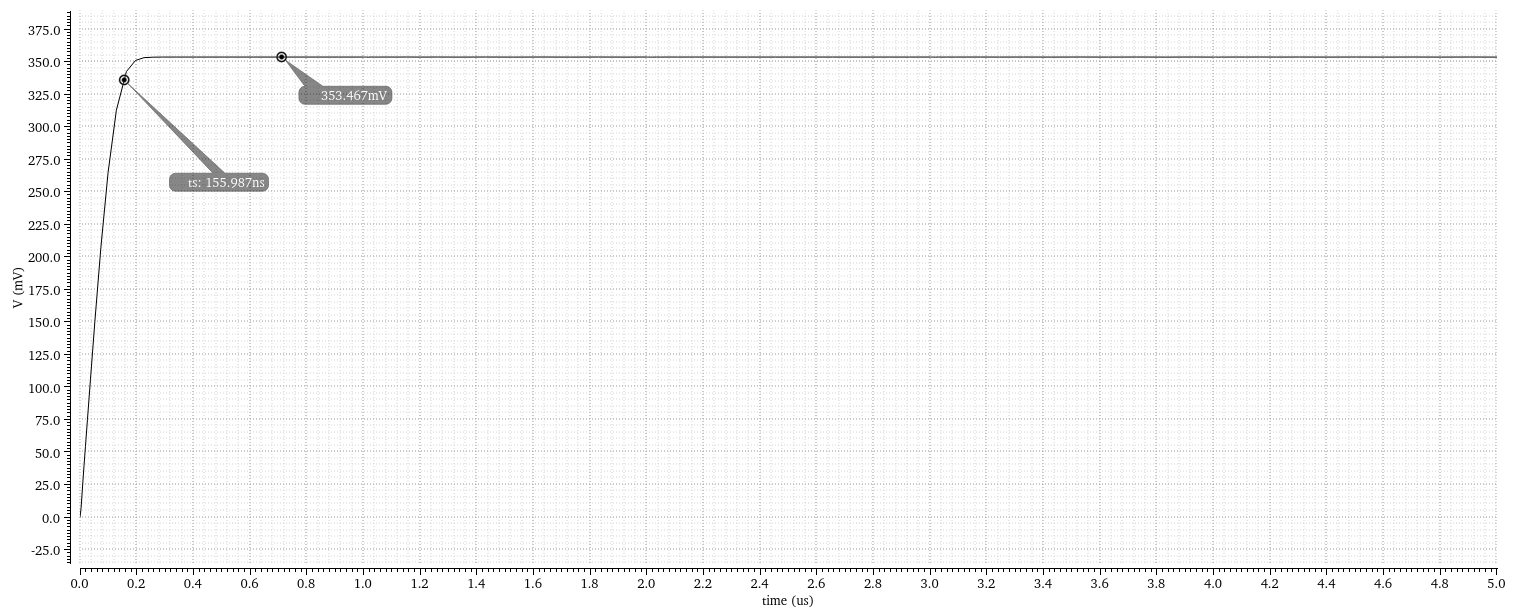
\includegraphics[width=0.85\textwidth]{immaginicorrettereport3/LOOP_DIFFERENTIAL_TRANSIENT.png}
    \caption{Transient response of the loop transfer function.}
    \label{fig:loop_transient}
\end{figure}

\subsection{Closed-Loop Feedback Amplifier Analysis}

The closed-loop differential transfer function of the capacitive feedback amplifier is plotted in Fig.~\ref{fig:closed_loop_bode}.

\begin{figure}[H]
    \centering
    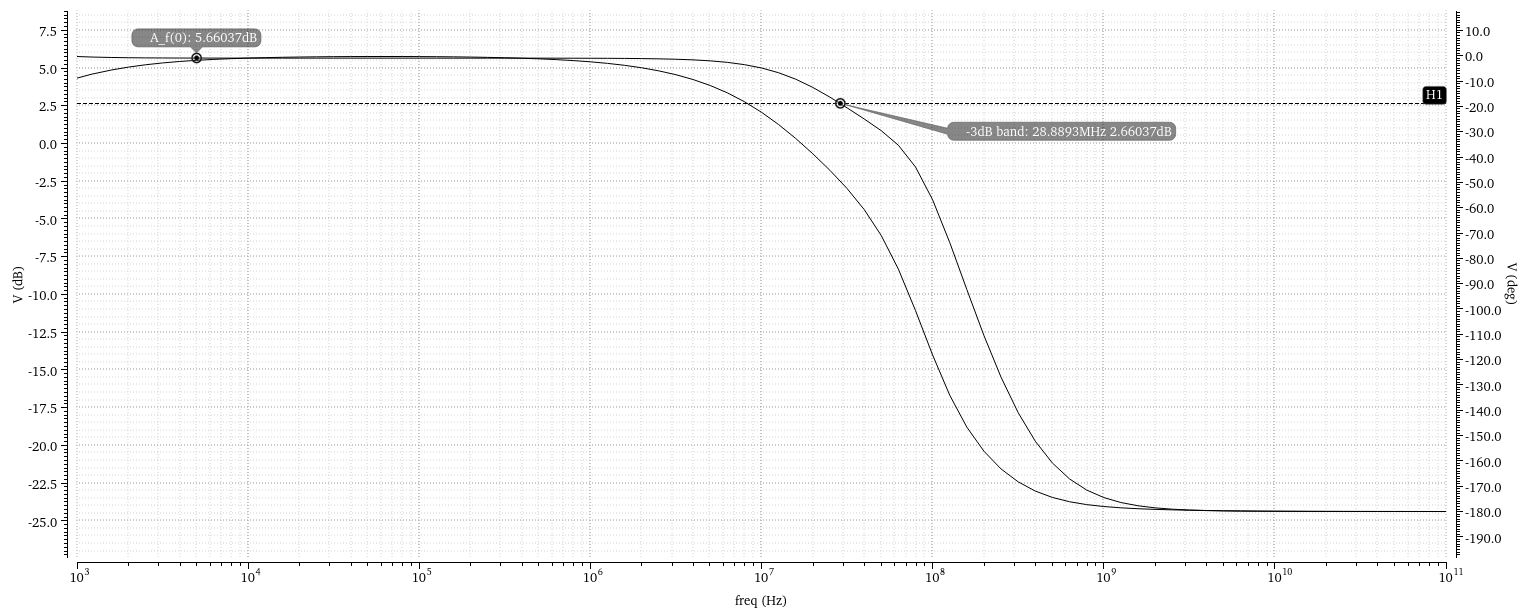
\includegraphics[width=0.85\textwidth]{immaginicorrettereport3/close_loop_differential.png}
    \caption{Bode plot of the closed-loop differential transfer function.}
    \label{fig:closed_loop_bode}
\end{figure}

The simulated low-frequency closed-loop gain is $A_{CL,0}=5.66\,\mathrm{dB}=1.92$. Compared to the ideal value set by the capacitive ratio ($A_{CL,ideal}=\frac{C_s}{C_f}=2$), the resulting static error is:
\[
\varepsilon_s= \left| \frac{A_{CL,ideal}-A_{CL,0}}{A_{CL,ideal}} \right| = \left| \frac{2-1.92}{2} \right| \simeq 4.1\%
\]
The measured $-3\,\mathrm{dB}$ bandwidth is $f_{-3\mathrm{dB}}\simeq28.89\,\mathrm{MHz}$.

\subsection{Closed-Loop Step Response and Dynamic Error}

\begin{figure}[H]
    \centering
    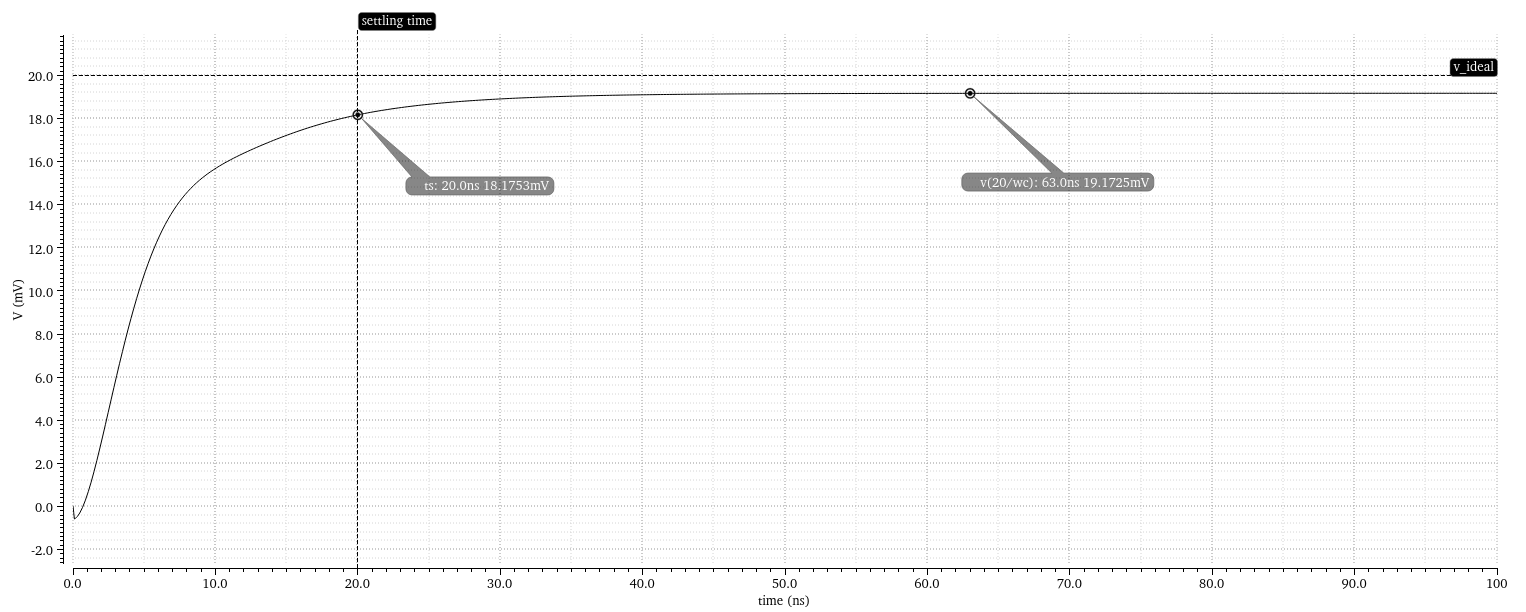
\includegraphics[width=0.85\textwidth]{immaginicorrettereport3/final_transient_response.png}
    \caption{Closed-loop differential step response of the final feedback amplifier.}
    \label{fig:closed_loop_transient}
\end{figure}

Fig.~\ref{fig:closed_loop_transient} shows the closed-loop step response to a $10\,\mathrm{mV}$ differential input step, where $V_{out,ideal}=20\,\mathrm{mV}$. The simulation reports $V_{out}(20\,\mathrm{ns})=18.175\,\mathrm{mV}$ and a settled value $V_{out}(\infty)\simeq19.173\,\mathrm{mV}$, yielding a dynamic error at $t_s=20\,\mathrm{ns}$ of:
\[
\varepsilon_d= \left| \frac{V_{out}(\infty)-V_{out}(20\,\mathrm{ns})}{V_{out}(\infty)} \right| = \frac{19.173-18.175}{19.173} \simeq 5.2\%
\]
This discrepancy arises because the theoretical first-order approximation $\varepsilon_d(t)\simeq e^{-\omega_c t}$ assumes a single dominant pole. In this OTA implementation, the second pole is close enough to the crossover frequency to introduce non-dominant exponential modes, slowing down the settling behavior and increasing the simulated dynamic error.



\subsection{Offset Voltage Estimation}

The OTA input-referred offset voltage was estimated via a 100-sample mismatch-only Monte Carlo simulation using the testbench shown in Fig.~\ref{fig:offset_tb}.

\begin{figure}[H]
    \centering
    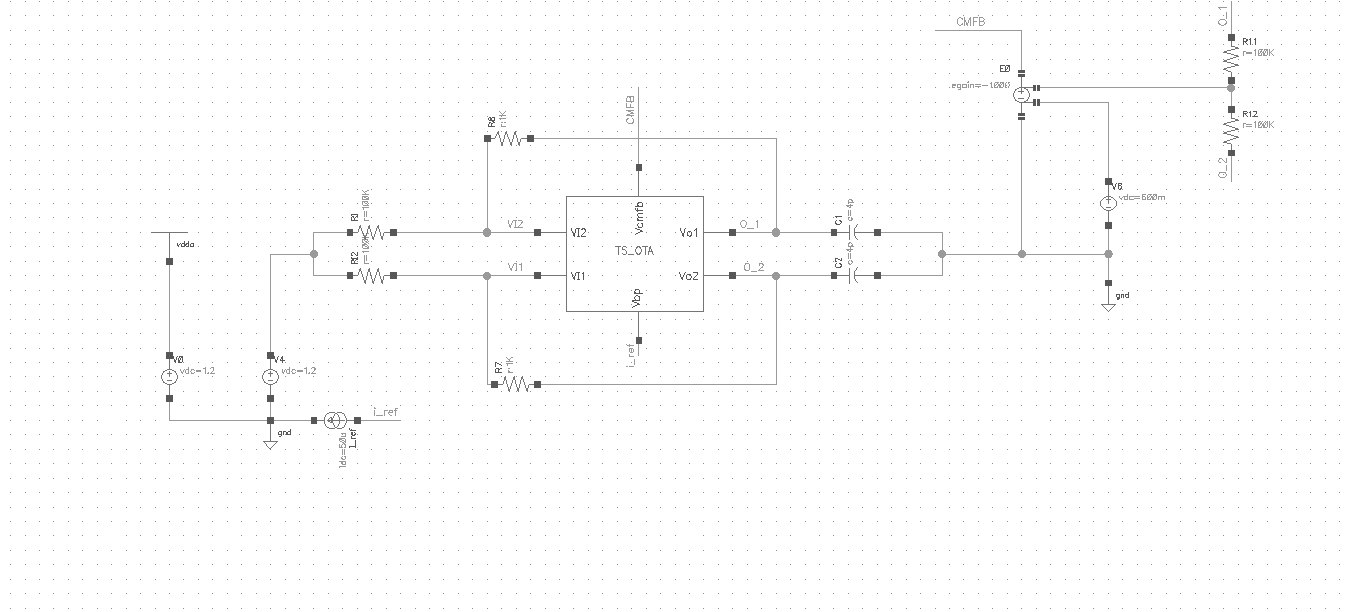
\includegraphics[width=0.85\textwidth]{immaginicorrettereport3/CORRECTMONTECARLO.png}
    \caption{Testbench employed for the Monte Carlo estimation of the input-referred offset voltage.}
    \label{fig:offset_tb}
\end{figure}

The resistive feedback network forces the OTA to operate close to equilibrium, while the high-gain loop minimizes the differential input voltage. Under the condition $\beta A_{dd0}\gg1$, the residual differential input voltage approximates the input-referred offset voltage:
\[
V_{ID}=V_{i2}-V_{i1}\approx V_{OS}
\]

The statistical distribution of the extracted differential input voltage is plotted in Fig.~\ref{fig:montecarlo_offset}.

\begin{figure}[H]
    \centering
    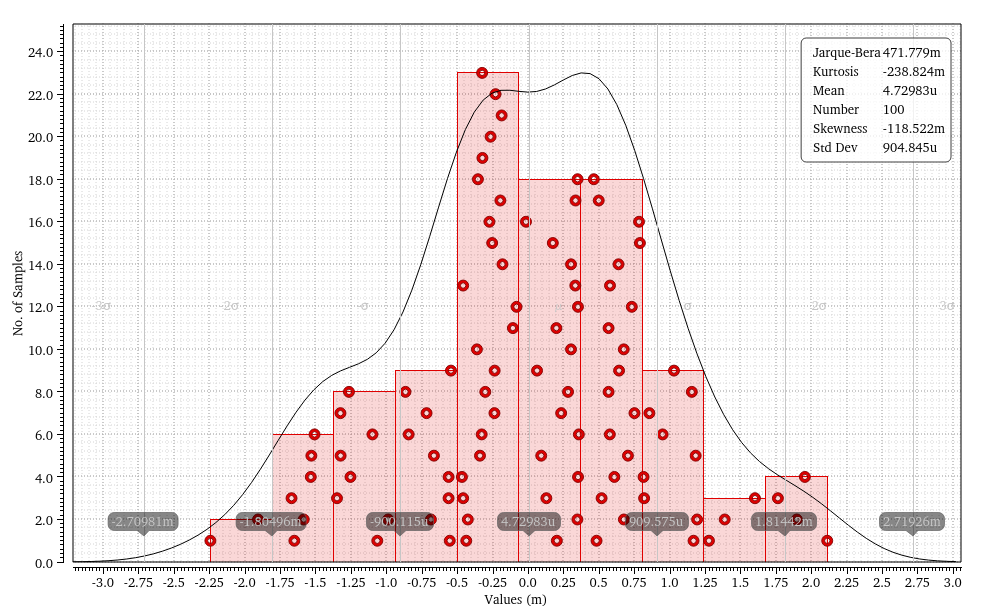
\includegraphics[width=0.85\textwidth]{immaginicorrettereport3/CORRECTMONTECARLONE.png}
    \caption{Monte Carlo distribution of the estimated input-referred offset voltage.}
    \label{fig:montecarlo_offset}
\end{figure}

The simulation yields a standard deviation of $\sigma(V_{ID})\simeq904.8\,\mu\mathrm{V}$. Therefore, the estimated input-referred offset voltage is:
\[
\boxed{V_{OS}\simeq0.905\,\mathrm{mV}}
\]
This complies with the design specification ($V_{OS}\leq2\,\mathrm{mV}$).
\section{Discussion of Unmet Specifications}

The final two-stage OTA design successfully optimized the trade-offs between speed, stability, and power consumption, satisfying the main specifications. The procedure was systematically developed from first-order analytical models, translating the static error target into a minimum loop gain ($\varepsilon_0\simeq\frac{1}{1+T_0}$) and the dynamic settling-time target into a minimum crossover frequency via the theoretical relation:
\[
\varepsilon_d(t_s)\simeq e^{-\omega_c t_s}
\]
This expression assumes an ideal first-order system where a single dominant pole governs the entire dynamics up to the crossover frequency.

The resulting system is not a simple single-pole network; consequently, the simulated closed-loop $-3\,\mathrm{dB}$ bandwidth ($f_{-3\mathrm{dB}}\simeq28.89\,\mathrm{MHz}$) deviated from the crossover frequency ($f_c\simeq50.51\,\mathrm{MHz}$). This non-ideality limited the settling behavior, causing the static error to settle at $4.1\%$ and the dynamic error at $5.2\%$, missing the highly conservative target of $0.2\%$. Pure first-order settling would ideally require a phase margin close to $90^\circ$ to completely suppress any non-dominant exponential mode. 


Moreover, the laboratory guidelines originally specified a required phase margin between $60^\circ$ and $70^\circ$. This initially motivated a compensation network targeting approximately $61.35^\circ$, yielding a moderately underdamped but fast transient response. After subsequent clarifications—obtained when the design and simulations were already completed—it was understood that the original specification contained an error and the intended requirement was a phase margin greater than $70^\circ$. This final interpretation is highly consistent with the theoretical framework of this report: a larger phase margin pushes the second pole higher, bringing the loop response closer to the dominant-pole behavior required by the first-order error equations.